Cette section montre le contenu initial de la base de données au début du projet, ainsi que les ajustements et ajouts effectués.

\section{Base de données initiale}

Voici le schéma de la base de données lors de la reprise du projet :

\begin{figure}[H]
    \begin{center}
        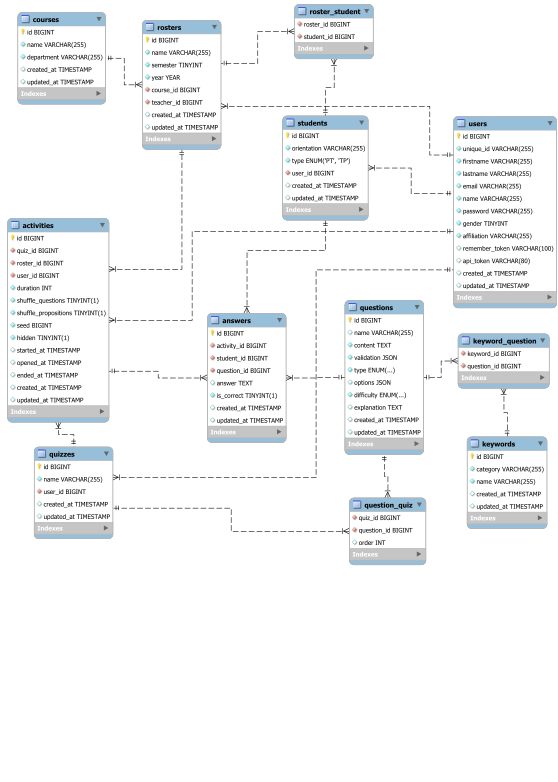
\includegraphics[width=14cm]{\assetsdir/diagramBaseDB.svg.pdf}
    \end{center}
    \caption[Diagramme de la base de données initiale]{\label{assembly}Diagramme de la base de données initiale}
\end{figure}

Il est donc nécessaire de modifier cette base de données afin qu'elle puisse répondre aux nouveaux besoins de l'application. De plus, quelques modifications seront effecutées afin d'éviter la redondance de données. Les détails de ces ajustements sont présentés dans les sections suivantes.

\section{Modifications apportées aux tables existantes}

\subsection{Table "users"}
Plusieurs modifications ont été effectuées dans cette table. Notamment, le champ "name" qui a été supprimé, car il était une concaténation des champs "firstname" et "lastname". Il convient donc de l'enlever afin d'éviter la redondance de données. Le champ \emph{unique\_id} devient \emph{keycloak\_id} et permet de savoir lors de la connexion si un utilisateur possède déjà un compte sur l'application ou si l'on doit le créer. Les champs \emph{password} et \emph{api\_token} sont quant à eux supprimés car plus nécessaire.

\subsection{Table "quizzes"}
La seule modification apportée à cette table est l'ajout d'un champ \emph{type} qui est une \emph{enum} comprenant les valeurs \emph{quiz} et \emph{exam}. Ce champ permet de différencier les quiz des examens.

\subsection{Table "questions"}
Le champ \emph{type} de cette table a été étendu afin d'ajouter la valeur \emph{long-answer} aux quatre autres valeurs déjà existantes (\emph{"short-answer", "fill-in-the-gaps", "multiple-choice"} et \emph{"code"}). Cette valeur permet de différencier les questions à développement des questions à réponse courte. L'ajout d'un \emph{user\_id} permet de connaître le créateur de la question et de restreindre la modification de la question uniquement à ce dernier. Cet ajout, lié au nouveau champ \emph{is\_public} permet de créer des questions privées qui ne pourront pas être utilisées par d'autres professeurs dans leurs quiz. De plus, l'ajout d'un champ concernant la visibilité de la question sera utile pour savoir quelles questions peuvent être sélectionnées dans le mode \emph{drill}. Enfin, l'ajout du champ \emph{points} permet d'attribuer un nombre de points à chaque question, ce qui est essentiel pour calculer le nombre total de points d'un examen ou d'un quiz.

\subsection{Table "answers"}
Un champ \emph{points} a également été ajouté à cette table, permettant de d'attribuer un certain nombre de points à la réponse d'un élève. Ce champ est utilisé pour calculer le nombre de points obtenus par un élève à un examen ou un quiz.

\section{Intégrité des données}
Avec l'ajout de travaux écrits sur la plateforme, la question de l'intégrité des données se pose. En effet, puisque les questions sont modifiables par leur créateur, il est alors possible qu'un enseignant modifie une question d'examen après que ce dernier se soit déroulé. Ce qui aurait des conséquences directes sur les réponses des élèves. Pour éviter cela, deux solutions sont envisagées.

La première solution consiste à fournir un \emph{hash} de l'examen et de toutes ses questions que les étudiants pourront comparer lors de la correction. Cette solution présente comme avantage la facilité de mise en place, mais a un énorme défaut. En effet, un examen peut contenir des questions créées par d'autres enseignants. Ces derniers pourraient donc modifier leurs questions indépendamment de la volonté de l'enseignant responsable de l'examen. Suite à la modification, la comparaison des deux hash nous dirait donc que l'examen a bien été modifié mais il serait impossible de savoir à quel point et que faire pour corriger cela.

La deuxième solution, plus compliquée à mettre en place, consiste à copier les questions de l'examen dans une table distincte. Cela va créer une certaine redondance des données, mais c'est la solution qui semble être le mieux adapté à notre situation. La copie des questions se ferait lors du lancement du quiz de type examen. Ensuite, lors de l'examen, l'application ira lire les questions dans cette table à part. Ainsi, si un enseignant modifie une question après le début de l'examen, cela n'aura aucune conséquence sur les réponses des élèves. Pour éviter au maximum la redondance de données, on ne copiera que les questions d'un quiz de type examen et non les questions des quiz normaux.

Cette deuxième solution est la plus adaptée à notre situation. Elle permet de garder l'intégrité des données tout en minimisant la redondance de ces dernières.

\section{Ajout de tables}

\subsection{Table activity\_student}
Cette table a été créée dans le but de savoir si l'étudiant a rendu un examen ou non. Lorsqu'un élève termine un quiz en avance, il peut le rendre. Cependant, s'il retourne sur l'activité, il peut continuer de répondre aux questions. Grâce à l'ajout de cette relation, il est désormais possible de savoir si l'étudiant effectivement rendu son examen, permettant ainsi de limiter son accès le cas échéant.

\subsection{Table exam\_questions}
Comme expliqué dans la section sur l'intégrité des données, cette table permet de faire une copie des questions d'un examen. Certains champs n'ont pas été copiés dans cette nouvelle table. En effet, des champs tels que \emph{is\_public} ou \emph{user\_id} ne sont pas pertinent à dupliquer, car leur modification n'aura pas d'impact sur les réponses des élèves. On peut noter que le champ \emph{user\_id} de la table \emph{exam\_questions} aurait également pu être abandonné. Actuellement, le créateur de la question ne peut pas être modifié via l'application. Cela pourrait cependant être une fonctionnalité supplémentaire. C'est pour garder l'information sur le "propriétaire" de la question que ce champ a été conservé.

\subsection{Table drills}
Cette table a été créée dans le but de gérer le mode \emph{drill} de l'application. Une section du chapitre suivant est dédiée à cette fonctionnalité, c'est pourquoi il n'y a pas le détail sur les champs secondaires. Les trois clés étrangères \emph{student\_id}, \emph{question\_id} et \emph{keyword\_id} sont essentielles pour récupérer toutes les questions publiques avec un mot-clé spécifique pour un étudiant donné. Ces clés permettent de savoir si l'étudiant a déjà répondu à une question avec un mot-clé particulier, afin d'adapter les prochaines occurrences en fonction de ses résultats.

\subsection{Diagramme de modification de la base de données}
Pour des raisons de clarté, ce schéma montre toutes les tables, mais n'affiche que les nouvelles relations. Un diagramme complet se trouve à la section suivante.

\begin{figure}[H]
    \begin{center}
        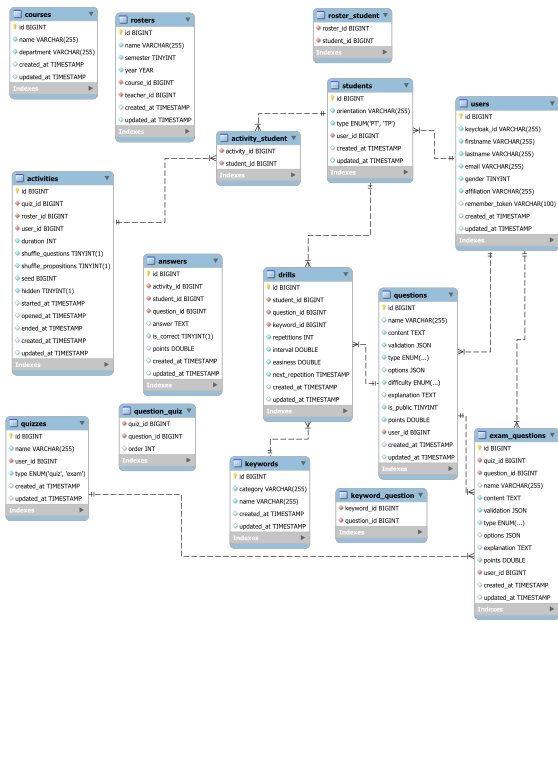
\includegraphics[width=14cm]{\assetsdir/diagramDBAdded.svg.pdf}
    \end{center}
    \caption[Diagramme des modifications de la base de données]{\label{assembly}Diagramme des modifications de la base de données}
\end{figure}

\section{Base de données finale}
Voici un schéma complet de la base de données après les modifications appliquées :
\begin{figure}[H]
    \begin{center}
        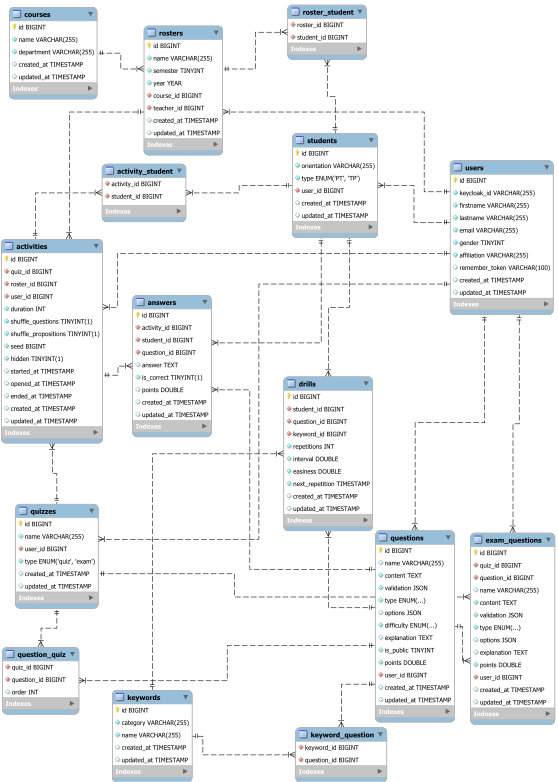
\includegraphics[width=14cm]{\assetsdir/digramDB.svg.pdf}
    \end{center}
    \caption[Diagramme de la base de données finale]{\label{assembly}Diagramme de la base de données finale}
\end{figure}